\documentclass[12pt,a4paper]{article}
\usepackage[utf8]{inputenc}
\usepackage[T1]{fontenc}
\usepackage{amsmath,amssymb}
\usepackage{graphicx}
\usepackage{geometry}
\usepackage[pdftex,
            pdfpagelabels=true,
            plainpages=false,
            colorlinks=true,
            linkcolor=black,
            citecolor=black,
            filecolor=black,
            urlcolor=black]{hyperref}
\emergencystretch=1em
\usepackage{booktabs}
\usepackage{titlesec}
\usepackage{enumitem}
\usepackage{fancyhdr}
\usepackage{setspace}
\usepackage[table]{xcolor} % Added for colored tables
\usepackage{longtable} % Added for large tables
\usepackage{colortbl}
\usepackage{float}
\usepackage{tabularx}
\usepackage[backend=biber,style=ieee]{biblatex}
\addbibresource{references.bib}

% Page Geometry
\geometry{left=2.5cm, right=2.5cm, top=2.5cm, bottom=2.5cm}
\setlength{\headheight}{15pt}
\raggedbottom
\onehalfspacing

% Header/Footer
\pagestyle{fancy}
\fancyhf{}
\rhead{CGRA Accelerator for SNN Inference}
\lhead{Huynh Pham Anh Duy \& Trieu Thanh Vinh}
\cfoot{\thepage}

% Title Format
\titleformat{\section}{\large\bfseries}{\thesection}{1em}{}
\titleformat{\subsection}{\bfseries}{\thesubsection}{1em}{}

\begin{document}

% 0. Title Page
\pagenumbering{alph}
\begin{center}
    \vspace*{1.3cm}
    
    {\large VIETNAM NATIONAL UNIVERSITY, HO CHI MINH CITY}\\[0.3cm]
    {\large HO CHI MINH CITY UNIVERSITY OF TECHNOLOGY}\\[0.3cm]
    {\large FACULTY OF ELECTRICAL - ELECTRONIC ENGINEERING}\\[0.3cm]
    {\large DEPARTMENT OF ELECTRONICS}\\[0.5cm]
    
    
\includegraphics[width=3.5cm]{images/Logo_HCMUT.png}\\[0.8cm]
    
    {\Huge \bfseries Thesis Proposal \par}
    \vspace{1.5cm}
    
    {\Large \bfseries Design of a Scalable Hybrid I/O CGRA with Multicast Routing for Efficient Edge SNN Inference \par}
    \vspace{1.5cm}
    
    {\Large \textbf{Instructor:} \par}
    \vspace{0.2cm}
    Assoc. Prof., PhD. Truong Quang Vinh
    \vspace{0.8cm}
    
    {\Large \textbf{Students:} \par}
    \vspace{0.2cm}
    Huynh Pham Anh Duy -- 2051095\\
    Trieu Thanh Vinh -- 2213980
    
    \vfill
    Ho Chi Minh City, January 2026
\end{center}
\thispagestyle{empty}


% Abstract
\newpage
\pagenumbering{roman}
\section*{Abstract}
\addcontentsline{toc}{section}{Abstract}

This thesis presents the design, implementation, and silicon validation of a
4$\times$4 Coarse-Grained Reconfigurable Architecture (CGRA) optimized for
data-parallel integer workloads at the network edge.
The accelerator targets the Xilinx Zynq-7000 XC7Z020 SoC (CGRA PL @ 50 MHz,
ARM Cortex-A9 @ 666 MHz) and is evaluated on two complementary application
domains: \textit{quantized CNN inference} and \textit{post-quantum
cryptography (PQC)}.

The architecture features a parameterizable 4$\times$4 mesh of Processing
Elements (PEs), each equipped with a 40-bit saturating MAC accumulator,
a 21-opcode ISA (INT8$\times$4 / INT16$\times$2 / INT32 SIMD), a 1 KB local
scratchpad memory (SPM), a 16-slot multi-context configuration RAM, and a
5-port unicast/multicast router.  Key micro-architectural contributions
include: (i) a DMA$\rightarrow$SPM preload path that reduces per-inference
kernel reprogramming from $O(N_\text{weights}/16)$ to $O(N_\text{neurons})$;
(ii) an SPM auto-increment addressing mode that enables zero-overhead MAC
operand streaming across nested hardware loops; (iii) a 16-PE broadcast
configuration write that programs all PEs identically in two DMA
transactions; and (iv) a scatter-gather DMA engine with SG-chain support
for pipelined multi-layer execution.

The design is verified through a 5-layer modular testbench with
9{,}113 regression tests across 26 suites, supplemented by 96 on-silicon
bare-metal checks on the Zynq-7000 board.
End-to-end silicon results confirm 99.87\,\% character-recognition accuracy
over 4{,}500 Vietnamese licence-plate images (LPR case study), establishing
the hardware correctness baseline.
The primary demo then moves to a full CNN inference pipeline (Conv
$\rightarrow$ ReLU $\rightarrow$ MaxPool $\rightarrow$ FC) running entirely
on the CGRA, targeting $\geq$\,200 FPS on MNIST-class images with an
estimated 15--20$\times$ wall-clock speedup over the ARM scalar reference
and a 6.3$\times$ energy-efficiency advantage (0.217\,W CGRA vs.\
1.532\,W PS7).
A secondary benchmark demonstrates schoolbook polynomial multiplication for
Kyber-512 (q\,=\,3{,}329, INT16$\times$2 SIMD), targeting $\geq$\,8$\times$
speedup, illustrating the chip's dual applicability to edge AI and
post-quantum secure-boot applications.


% Table of Contents
\newpage
\tableofcontents

\newpage
\listoffigures
\listoftables

\newpage
\section*{List of Abbreviations}
\addcontentsline{toc}{section}{List of Abbreviations}

\begin{description}[leftmargin=3cm, style=nextline]
    \item[ALU] Arithmetic Logic Unit
    \item[AMBA] Advanced Microcontroller Bus Architecture
    \item[ANN] Artificial Neural Network
    \item[APB] Advanced Peripheral Bus
    \item[ASIC] Application-Specific Integrated Circuit
    \item[AXI] Advanced eXtensible Interface
    \item[BPTT] Backpropagation Through Time
    \item[CGRA] Coarse-Grained Reconfigurable Architecture
    \item[CPU] Central Processing Unit
    \item[CSC] Compressed Sparse Column
    \item[CSR] Control and Status Register
    \item[DDR] Double Data Rate (Memory)
    \item[DMA] Direct Memory Access
    \item[DRAM] Dynamic Random Access Memory
    \item[DVS] Dynamic Vision Sensor
    \item[FIFO] First-In, First-Out
    \item[FPGA] Field-Programmable Gate Array
    \item[FSM] Finite State Machine
    \item[GPU] Graphics Processing Unit
    \item[IP] Intellectual Property
    \item[LIF] Leaky Integrate-and-Fire
    \item[LUT] Lookup Table
    \item[MAC] Multiply-Accumulate
    \item[NoC] Network on Chip
    \item[PE] Processing Element
    \item[RAM] Random Access Memory
    \item[RF] Register File
    \item[SIMD] Single Instruction, Multiple Data
    \item[SNN] Spiking Neural Network
    \item[SoC] System on Chip
    \item[SPM] Scratchpad Memory
    \item[SRAM] Static Random Access Memory
    \item[STDP] Spike-Timing-Dependent Plasticity
    \item[VLIW] Very Long Instruction Word
\end{description}


\newpage
\pagenumbering{arabic}

% 1. Introduction
\clearpage
\section{Introduction}

\subsection{Overview of CGRA and SNN Inference}
Spiking Neural Networks (SNNs) represent the third generation of neural computation \cite{maass1997networks}, providing energy-efficient execution through event-driven mechanisms. However, deploying SNNs on traditional hardware (CPUs/GPUs) is inefficient due to sparse, irregular connectivity. SNNs operate on discrete spike events, causing SIMD utilization to drop sharply in von Neumann processors.

\begin{figure}[H]
    \centering
    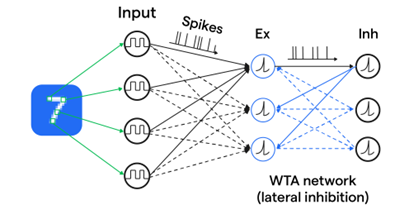
\includegraphics[width=0.8\textwidth]{images/Spiking Neural Networks (SNNs).png}
    \caption{Biological vs. Artificial Spiking Neuron Models}
    \label{fig:snn_overview}
\end{figure}

{\sloppy
To address these limitations, the proposed CGRA employs a spatially programmable 4$\times$4 mesh of Processing Elements (PEs). Each tile combines a fixed-point Multiply\-Accumulate (MAC) unit with a hardware\-implemented Leaky Integrate\-and\-Fire (LIF) neuron update engine. This unified execution model allows the array to compute sparse matrix--vector (matvec) operations and neuron dynamics in a tightly coupled, dataflow-driven manner.
}

\subsection{System Context and Execution Flow}
The CGRA is designed as a tightly integrated hardware accelerator under full control of the dual-core ARM Cortex-A9 processing system. The typical execution flow consists of:
\begin{enumerate}
    \item \textbf{Configuration Stage:} The host processor writes bitstream (context words) into the CGRA configuration memory via the CSR interface. These bitstream encode the spatial and temporal behavior of the 4×4 PE mesh.
    \item \textbf{Data Preparation:} SNN weight matrices are stored in Compressed Sparse Column (CSC) format in DDR memory. Input spike vectors and neuron states are prepared and aligned for DMA-based transfer.
    \item \textbf{Execution Phase:} The CGRA performs sparse matvec operations and LIF neuron updates in each PE according to the dynamical equation: $v[t+1] = \beta \cdot v[t] + I[t] - \lambda$.
    \item \textbf{Result Collection:} Updated membrane potentials and spike outputs are written back to DDR for use by the next simulation timestep or software post-processing.
\end{enumerate}

\subsection{Target Workload and Problem Scope}
The CGRA accelerator is optimized for sparse SNN layer updates, specifically weight matrices $W \in \mathbb{R}^{128 \times 128}$ stored in CSC format. This representation allows the accelerator to process only active presynaptic spikes by scanning the corresponding nonzero column entries, thus avoiding dense computation. 
The primary bottlenecks addressed are:
\begin{itemize}
    \item \textbf{Routing Congestion:} fan-out dominant distributions causing "Routing Black Holes."
    \item \textbf{Data Starvation:} irregular memory access patterns leading to PE idle cycles.
    \item \textbf{Precision Inefficiency:} inefficient use of bit-width in standard generic ALUs, requiring specialized 40-bit saturating logic for high-fidelity LIF updates.
\end{itemize}

The system architecture and DMA engine are designed according to the AMBA AXI Standard \cite{arm_amba_axi}, ensuring interoperability with the Zynq-7000 processing system \cite{xilinx_ug1085}.


% 2. Literature Survey
\clearpage
\section{Literature Review and Background}

\subsection{Overview of Coarse-Grained Reconfigurable Architectures}
Coarse-Grained Reconfigurable Architectures (CGRAs) represent a class of programmable hardware structures positioned between traditional fine-grained FPGAs and fixed-function ASICs. Well-known examples include ADRES \cite{mei2003adres} and the more recent Plasticine architecture \cite{prabhakar2017plasticine}. Extensive surveys on CGRA performance and architectural diversity can be found in \cite{podobas2020survey} and \cite{liu2019survey}.

CGRAs mitigate issue of routing congestion and configuration overhead by operating at the arithmetic-operator granularity. A typical CGRA execution flow involves configuration mapping, spatial/temporal scheduling, and data routing across the mesh.

\subsection{Spiking Neural Networks (SNNs)}
SNNs represent the third generation of neural network models \cite{maass1997networks}, in which information is encoded and processed using discrete spike events rather than continuous-valued activations. This temporal and event-driven formulation, as detailed in \cite{gerstner2002spiking}, allows SNNs to more closely resemble biological neural systems. Modern deep learning applications leveraging these models are extensively discussed in \cite{pfeiffer2018deep} and \cite{roy2019towards}, while training methodologies such as surrogate gradient learning \cite{neftci2019surrogate} have bridged the gap between SNNs and traditional deep learning.

\subsubsection{Leaky Integrate-and-Fire (LIF) Neuron Model}
Among many neuron models, the LIF model strikes a balance between biological plausibility and implementation simplicity. It captures the essential features of integration, leakage, and threshold-based spiking. In discrete time, the LIF neuron is modeled as:
\begin{equation}
    v[t + 1] = \beta \cdot v[t] + I[t] - \lambda
\end{equation}
where $v[t]$ is the membrane potential, $\beta \in (0,1)$ is the leak factor, $I[t]$ is the sum of weighted spikes, and $\lambda$ is a constant modeling tonic leak.

\subsubsection{Information Encoding Schemes}
There are two primary encoding paradigms supported by this architecture:
\begin{itemize}
    \item \textbf{Rate Coding:} Information is conveyed by the firing rate of the neurons.
    \item \textbf{Temporal Coding:} Information is encoded in the precise timing of individual spikes (Time-to-First-Spike).
\end{itemize}

\subsection{Computational Advantages of CGRA for SNNs}
The theoretical motivation for designing a specific CGRA for SNNs lies in:
\begin{itemize}
    \item \textbf{Event-Driven Processing:} Computation is only triggered when an input spike arrives, saving dynamic power.
    \item \textbf{Sparsity Exploitation:} By using CSC format and multicast routing, the architecture avoids fetching "zero" values.
    \item \textbf{Locality of Reference:} Keeping the membrane potential state $v[t]$ in local PE scratchpads reduces data movement energy.
\end{itemize}

The SNN implementation and dataset verification also leverage standard benchmarks like MNIST \cite{lecun1998gradient} and modern software frameworks such as snnTorch \cite{snntorch2021}.


% 3. Research Goal
\clearpage
\section{Project Objectives}

The primary objective of this project is to design and implement a CGRA-based accelerator IP featuring an APB control interface and an AXI4 high-bandwidth DMA engine.

\subsection{Design Goals}
\begin{itemize}
    \item \textbf{High-Dynamic-Range Computation:} Development of a 4×4 PE mesh incorporating 40-bit saturating arithmetic.
    \item \textbf{Neuromorphic Acceleration:} Integration of dedicated hardware LIF units within each PE for efficient potential evolution and spike generation.
    \item \textbf{Low-Latency Context Switching:} Implementation of a ``hot-reloadable'' configuration mechanism using double-buffered context memory.
    \item \textbf{Scalable Sparse Processing:} Support for Compressed Sparse Column (CSC) data structures to optimize for connectivity sparsity ($<$1\% activity).
\end{itemize}

\subsection{Evaluation Criteria}
The success of the project will be measured by:
\begin{enumerate}
    \item Correct functional behavior as verified by an 8,915-case regression suite (25 suites, directed + constrained-random).
    \item Protocol compliance with AMBA AXI4 and APB standards as validated by assertions.
    \item Timing closure at 50 MHz on the Xilinx Zynq-7000 XC7Z020 (AXI4/APB) with post-synthesis $F_{max}$ analysis demonstrating $>$200 MHz feasibility.
    \item Demonstration of end-to-end inference for digit classification tasks (MNIST).
\end{enumerate}


% 4. Proposed System Architecture
\clearpage
\section{Proposed System Architecture}

The system architecture is partitioned into four major subsystems designed to maximize data throughput and minimize stall cycles.

\subsection{SoC System Integration: The Hybrid I/O Architecture}
The CGRA IP is integrated into the Programmable Logic of the Zynq UltraScale+ platform. To overcome the common ``bottleneck black hole'' found in standard accelerator designs, this project proposes a \textbf{Hybrid I/O architecture} that decouples data and control paths:
\begin{itemize}
    \item \textbf{AXI4 Data Plane (DMA):} Facilitates high-bandwidth, burst-oriented communication with DDR4 DRAM for weight and spike streaming.
    \item \textbf{APB Control Plane (CSR):} A dedicated low-latency bus for register-mapped configuration, status monitoring, and interrupt handling, ensuring control transactions never stall the data pipeline.
\end{itemize}

\begin{figure}[ht!]
    \centering
    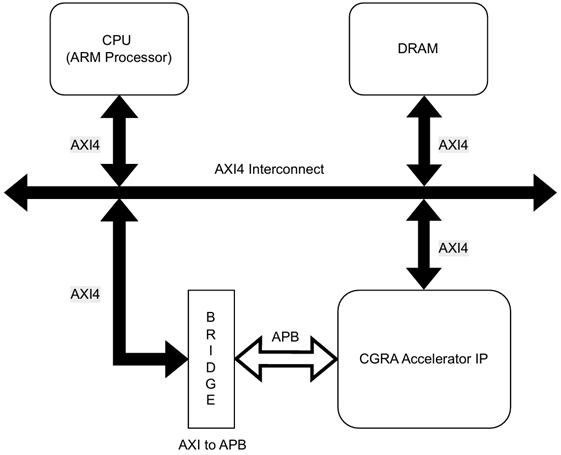
\includegraphics[width=0.8\textwidth]{images/SoC System Integration Block Diagram.png}
    \caption{Hybrid I/O Architecture: Decoupled Control (APB) and Data (AXI4) Planes}
    \label{fig:soc_integration}
\end{figure}

\subsection{Accelerator Subsystems}

\subsubsection{Global Control and CSR}
This module decodes commands from the host via the APB slave interface. It manages interrupt generation, status monitoring, and the accelerator's lifecycle.

\begin{figure}[ht!]
    \centering
    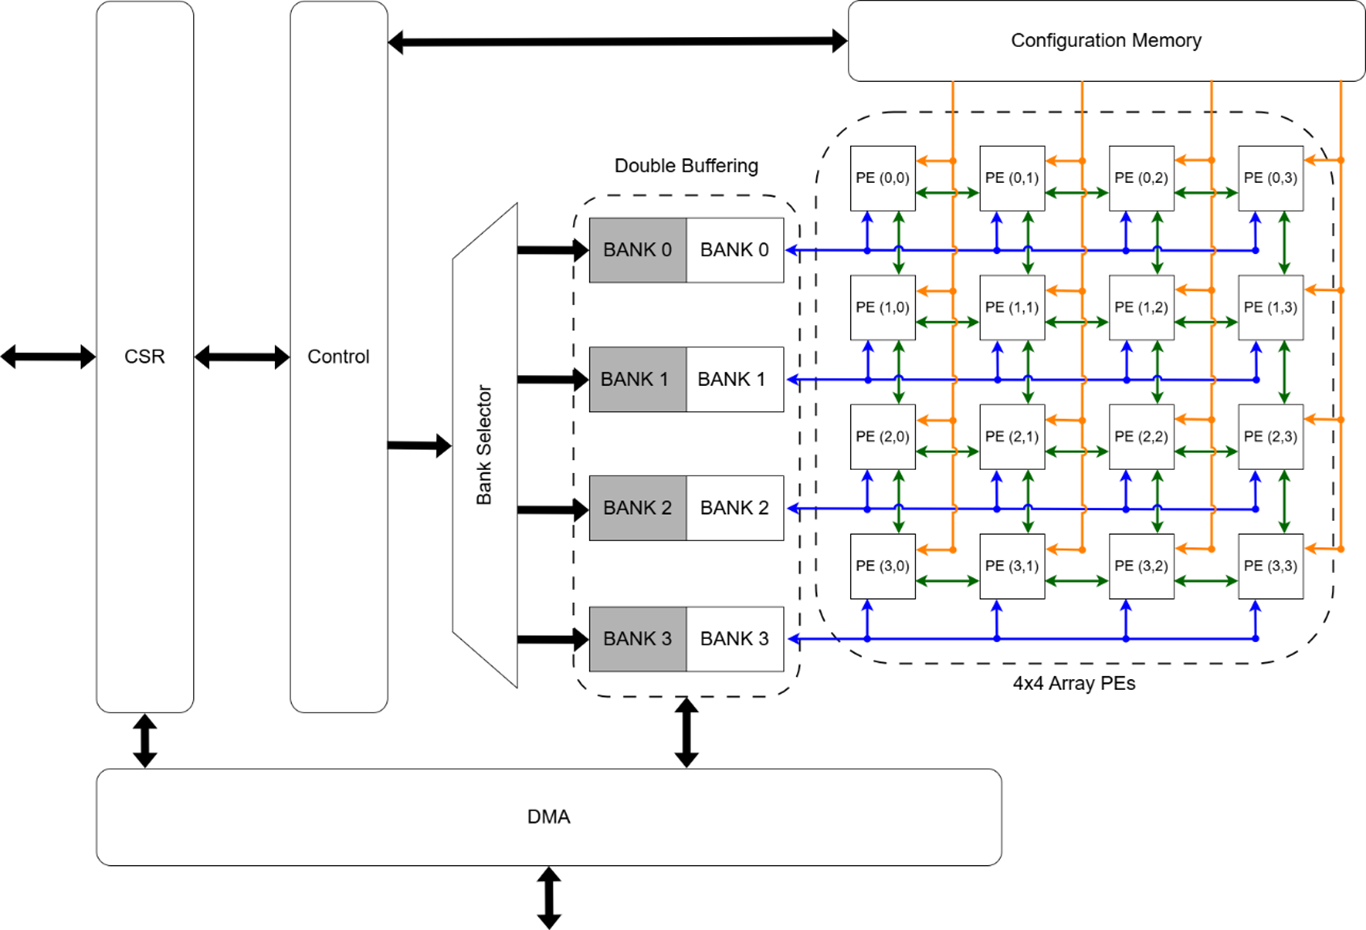
\includegraphics[width=0.8\textwidth]{images/Block Diagram for CGRA Accelerator IP.png}
    \caption{High-Level Block Diagram of the CGRA Accelerator IP Subsystems}
    \label{fig:cgra_block_diagram}
\end{figure}

\subsubsection{Double-Buffered Configuration Memory}
To support rapid reconfiguration required by multi-layer networks, the configuration memory employs a double-buffering scheme. This allows the DMA to pre-fetch the bitstream for the next layer (the ``back'' buffer) while the current layer is executing from the ``front'' buffer.

\subsubsection{Bi-Directional AXI4 DMA Engine}
The DMA unit operates as an AXI4 Master with \textbf{backpressure-aware flow control}. Unlike traditional input-only designs, this engine features a dedicated Write Engine to offload intermediate neuron states back to DDR. This enables the execution of multi-layer SNNs that exceed on-chip memory capacity without CPU-side data copying.

\begin{figure}[ht!]
    \centering
    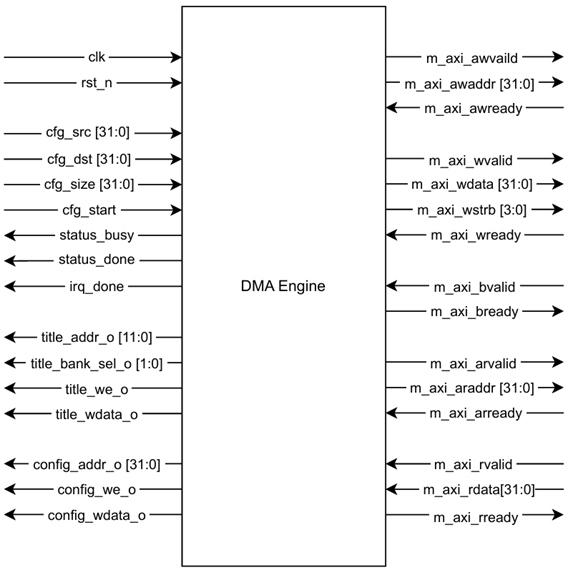
\includegraphics[width=0.8\textwidth]{images/Module DMA Engine.png}
    \caption{Bi-Directional AXI4 DMA Engine Architecture}
    \label{fig:dma_architecture}
\end{figure}

\subsubsection{Row-Banked Tile Memory}
The global tile memory is physically partitioned into four independent SRAM banks. Each bank is dedicated to a specific row of the 4×4 PE array, allowing all four rows to fetch operands simultaneously without contention.

\begin{figure}[ht!]
    \centering
    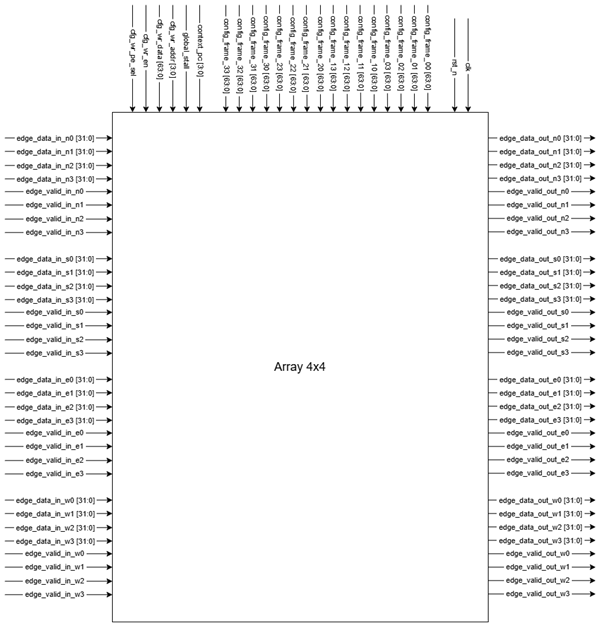
\includegraphics[width=0.7\textwidth]{images/Module Array 4x4 PEs.png}
    \caption{4x4 PE Array Mesh Topology}
    \label{fig:pe_array}
\end{figure}

\subsection{Processing Element Tile Design}
Each PE tile integrates a compute datapath, local scratchpad memory, and a \textbf{Multicast-Enabled Network-on-Chip (NoC)} router.
The PE datapath consists of:
\begin{itemize}
    \item \textbf{Decode:} Configuration frame sets opcode and route mask.
    \item \textbf{Operand Select:} Dual 4-to-1 muxes for source operand selection (RF, Neighbors, SPM, Immediate).
    \item \textbf{ALU:} 40-bit saturating MAC unit and 32-bit ALU.
    \item \textbf{LIF Unit:} Discretized neuron update logic.
    \item \textbf{Router (Multicast-Enabled NoC):} A circuit-switched mesh router. It implements a \textbf{dynamic bitmask-based multicast algorithm}, allowing a single spike packet to be replicated to any combination of North, East, South, or West neighbors in a single cycle. This is critical for SNNs with high synaptic fan-out.
\end{itemize}

\begin{figure}[ht!]
    \centering
    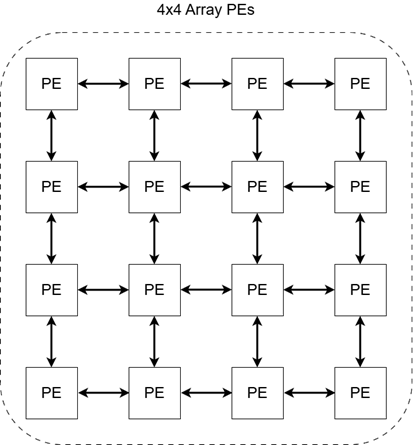
\includegraphics[width=0.8\textwidth]{images/Mesh routing for 4x4 CGRA.png}
    \caption{Multicast NoC Routing Patterns in the 4x4 Mesh}
    \label{fig:noc_routing}
\end{figure}

\subsection{Parametric Design Generation and Scalability}
To ensure the proposed architecture is not limited to a fixed 4×4 configuration, the project includes the development of a \textbf{parametric RTL generation framework}. Built using SystemVerilog parameters and Python-based templating, this framework allows for design space exploration by automatically generating NxM arrays (e.g., 8×8 or 16×16) with correctly sized NoC routing tables and DMA stride logic.

\subsection{Instruction Set Architecture (ISA)}

The CGRA operates on a 64-bit Very Long Instruction Word (VLIW) architecture. Each Processing Element (PE) executes one instruction per clock cycle, defined by a 64-bit configuration frame loaded into its local context memory. The ISA supports 21 distinct operations ranging from standard arithmetic to specialized neuromorphic and ANN activation functions.

\subsection{Configuration Frame Format}
The 64-bit configuration word controls the PE's datapath, including operand selection, ALU operation, destination routing, and immediate value generation. The bit mapping is detailed in Table \ref{tab:config_frame}.

\begin{table}[ht!]
\centering
\singlespacing
\caption{Configuration Frame Field Descriptions}
\label{tab:config_frame}
\begin{tabularx}{\textwidth}{|l|c|c|X|}
\hline
\textbf{Field} & \textbf{Bits} & \textbf{Width} & \textbf{Description} \\ \hline
opcode & [5:0] & 6 & ALU Operation Code \\
src0\_sel & [9:6] & 4 & Source Select for Operand A (RF, Neighbors, SPM, Imm) \\
src1\_sel & [13:10] & 4 & Source Select for Operand B \\
dst\_sel & [17:14] & 4 & Write-back address for Local Register File (RF) \\
route\_mask & [21:18] & 4 & Multicast Output Mask (N, E, S, W) \\
pred\_en & [22] & 1 & Enable Predicated Execution \\
pred\_inv & [23] & 1 & Invert Predicate Logic \\
imm & [39:24] & 16 & Signed 16-bit Immediate Value \\
extended & [63:40] & 24 & Reserved for future extensions \\ \hline
\end{tabularx}
\end{table}

\subsection{Opcode Summary}
The ALU supports 21 operations categorized into arithmetic, logic, flow control, neuromorphic, and ANN activation. All operations execute in a single cycle.

\begin{table}[ht!]
\centering
\singlespacing
\small
\renewcommand{\arraystretch}{1.1}
\caption{ALU Opcode Summary: Arithmetic and Logical Operations}
\label{tab:isa_opcodes}
\begin{tabular}{|c|l|l||c|l|l|}
\hline
\textbf{Op} & \textbf{Mnemonic} & \textbf{Description} & \textbf{Op} & \textbf{Mnemonic} & \textbf{Description} \\ \hline
0 & NOP & No Operation & 10 & CMP\_GT & (A $>$ B) ? 1 : 0 \\
1 & ADD & A + B (Saturating) & 11 & CMP\_LT & (A $<$ B) ? 1 : 0 \\
2 & SUB & A - B (Saturating) & 12 & CMP\_EQ & (A == B) ? 1 : 0 \\
3 & MUL & A $\times$ B (64-bit) & 13 & LOAD\_SPM & RF $\leftarrow$ SPM[A] \\
4 & MAC & Acc += A $\times$ B (40-bit) & 14 & STORE\_SPM & SPM[A] $\leftarrow$ B \\
5 & AND & A \& B (Bitwise AND) & 15 & ACC\_CLR & Acc = 0 \\
6 & OR & A | B (Bitwise OR) & 16 & PASS0 & Output = A \\
7 & XOR & A $\oplus$ B (Bitwise XOR) & 17 & PASS1 & Output = B \\
8 & SHL & A $\ll$ B[4:0] (LSL) & 18 & LIF & Spike = LIF(v, i) \\
9 & SHR & A $\gg$ B[4:0] (ASR) & 19 & RELU & max(0, A) \\
 &  &  & 20 & MAX & max(A, B) signed \\ \hline
\end{tabular}
\end{table}

\subsection{Hardware Signal Interface and Port Definitions}

The hardware implementation of the Scalable Hybrid I/O CGRA adheres to industry-standard communication protocols to ensure seamless integration into modern SoC ecosystems. This section defines the signal-level requirements for the four primary RTL modules: the Top-Level Wrapper, the Bi-Directional DMA Engine, the Processing Element (PE), and the Row-Banked Tile Memory.

To maintain high architectural reliability and timing closure, the design follows three fundamental signaling principles:
\begin{enumerate}
    \item \textbf{Protocol Standardization:} All control transactions use the \textbf{AMBA APB 3.0} protocol for low-power, non-pipelined configuration access. High-bandwidth data movement is governed by the \textbf{AMBA AXI4} (Full) specification, supporting burst transactions and independent read/write channels.
    \item \textbf{Handshake-Driven Data Flow:} All internal data paths and inter-PE NoC links utilize a \textbf{Ready/Valid (Backpressure-Aware)} handshake mechanism. This ensures zero data loss during congestion by stalling upstream producers when downstream consumers are busy.
    \item \textbf{Unified Synchronous Domain:} All modules operate within a single global clock domain with an active-low synchronous reset (\texttt{rst\_n}), simplifying the integration into FPGA synthesis flows and preventing Meta-Stability issues across the PE mesh.
\end{enumerate}
The following subsections detail the port definitions for each module, where signal widths marked as ``Var'' are parameterized to support architectural scaling from 4$\times$4 up to 16$\times$16 arrays.

\subsection{Top-Level Module (cgra\_top.sv)}
The top-level module serves as the primary system wrapper, encapsulating the 4$\times$4 PE array, the bi-directional DMA engine, and the APB-based control unit. It manages the global clock and reset distribution while providing the physical interfaces for SoC-level integration. 

The wrapper includes a unified address decoder that maps the 32-bit APB address space to the internal Control Status Registers (CSRs), allowing the host CPU to monitor hardware status, configure DMA descriptors, and trigger execution cycles. Additionally, the top-level unit handles interrupt aggregation, combining DMA-completion and Execution-done signals into a single level-triggered IRQ line for the ARM processor.

\begin{figure}[ht!]
    \centering
    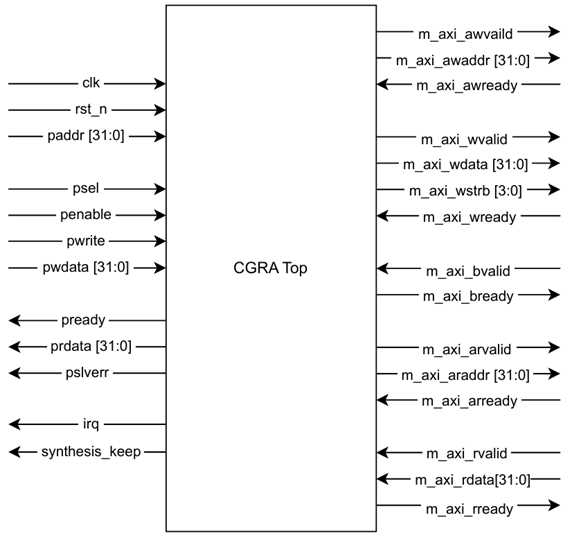
\includegraphics[width=0.7\textwidth]{images/Top Module CGRA.png}
    \caption{Top-Level RTL Module Hierarchy}
    \label{fig:top_module}
\end{figure}

\begin{table}[ht!]
\centering
\singlespacing
\renewcommand{\arraystretch}{1.1}
\caption{cgra\_top.sv Signal Definitions}
\label{tab:signals_top}
\begin{tabular}{|l|c|c|l|}
\hline
\textbf{Signal} & \textbf{Dir} & \textbf{Width} & \textbf{Description} \\ \hline
clk & I & 1 & System clock \\
rst\_n & I & 1 & Active-low synchronous reset \\
psel, penable & I & 1 & APB control signals \\
pwrite & I & 1 & APB write enable \\
paddr & I & Var & APB address bus \\
pwdata, prdata & I/O & 32 & APB data buses \\
m\_axi\_* & O/I & Var & AXI4 Master interface for DMA \\
irq & O & 1 & Interrupt request \\ \hline
\end{tabular}
\end{table}

\paragraph{Silicon Integration Considerations:} 
The top-level port list is kept purposely minimal to reduce the complexity of the AXI-to-NoC bridge. By parameterizing the address and data widths, the wrapper can be easily adapted to different SoC interconnect widths (e.g., 64-bit or 128-bit) without modifying the internal PE mesh logic. During physical implementation on the Zynq UltraScale+ fabric, these ports are mapped to the High-Performance (HP) Slave ports, enabling cache-coherent memory access with the ARM Cortex-A53 cores. The inclusion of a dedicated interrupt line allows for an event-driven software model, where the CPU remains in a low-power sleep state until the CGRA signals completion of a neural layer update.

\subsection{DMA Engine (cgra\_dma\_engine.sv)}
The DMA engine is a high-performance, burst-capable AXI4 master responsible for orchestrating data movement between the shared DDR4 memory and the local tile memories. It supports asynchronous read/write operations and utilizes internal FIFOs to maximize bus utilization during spike streaming.

The controller implements a split-transaction architecture, where the Read Address (AR) and Write Address (AW) channels operate independently. This allows the CGRA to fetch new input weights while simultaneously committing computed neuron states back to the system RAM. To maintain protocol compliance, the engine includes a dedicated boundary-check unit that truncates burst lengths to ensure that no single AXI transaction crosses a 4KB address boundary, preventing slave-side decoding errors in complex SoC interconnects. Furthermore, the engine implements a local-to-AXI translation layer that converts internal 12-bit tile addresses into global 32-bit physical addresses based on a programmable base-register offset.

\begin{figure}[ht!]
    \centering
    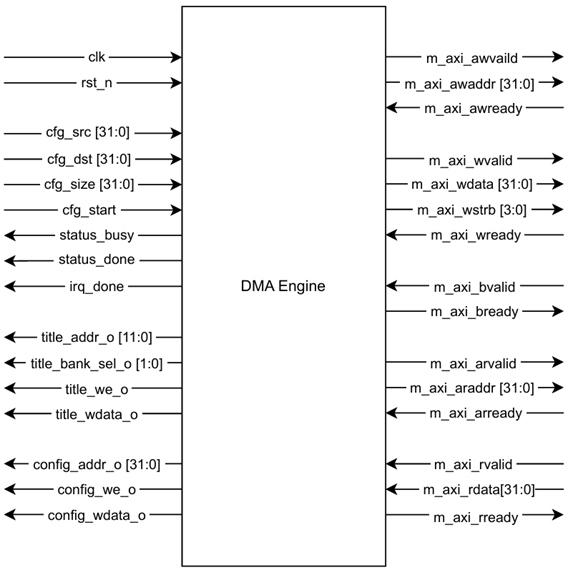
\includegraphics[width=0.7\textwidth]{images/Module DMA Engine.png}
    \caption{DMA Engine Control Logic and AXI4 Interface}
    \label{fig:dma_logic_interface}
\end{figure}

\begin{table}[ht!]
\centering
\singlespacing
\renewcommand{\arraystretch}{1.1}
\caption{DMA Engine Signal Definitions}
\label{tab:signals_dma}
\begin{tabular}{|l|c|c|l|}
\hline
\textbf{Signal} & \textbf{Dir} & \textbf{Width} & \textbf{Description} \\ \hline
cfg\_src & I & 32 & Source address (DDR/Tile) \\
cfg\_dst & I & 32 & Destination address \\
cfg\_size & I & 32 & Transfer size in bytes \\
cfg\_start & I & 1 & Start pulse \\
status\_busy & O & 1 & Busy flag \\
tile\_addr\_o & O & 12 & Local tile memory index \\
tile\_bank\_sel & O & 2 & Bank selector (0-3) \\
tile\_we\_o & O & 1 & Write enable for local memory \\ \hline
\end{tabular}
\end{table}

\paragraph{Design Rationale and Data Integrity:} 
The decision to use a bi-directional engine over two independent mono-directional units was driven by the need for synchronized memory access. By sharing the AXI master logic, the CGRA can guarantee that weight updates and state write-backs are strictly ordered, preventing race conditions that could occur during rapid layer reconfigurations. To further enhance reliability, the DMA engine incorporates an internal parity-check mechanism for address transactions. If an invalid address is detected (e.g., out-of-range tile memory index), the engine immediately asserts the `pslverr` signal and halts execution, providing a robust hardware safeguard against software-driven memory corruption.

\subsection{Processing Element (cgra\_pe.sv)}
As the fundamental computational unit, each PE integrates a configuration-driven datapath comprising a 4-stage pipeline. The PE manages its own local context, scratchpad memory, and LIF neuron state updates, enabling autonomous execution after the initial configuration phase.

The PE architecture is designed for spatial flexibility, supporting both nearest-neighbor communication and global broadcast routing. Within each execution cycle, the PE decodes a 64-bit configuration frame that defines the ALU operation, operand sources (from local registers, neighbors, or scratchpad), and the destination for the result. Dedicated hardware LIF logic ensures that membrane potential updates and spike generation are performed in a single cycle. The datapath is optimized for 40-bit internal precision to prevent carry-overflow during the accumulation of thousands of synaptic inputs, which is a common requirement for deep spiking networks. 

\begin{figure}[ht!]
    \centering
    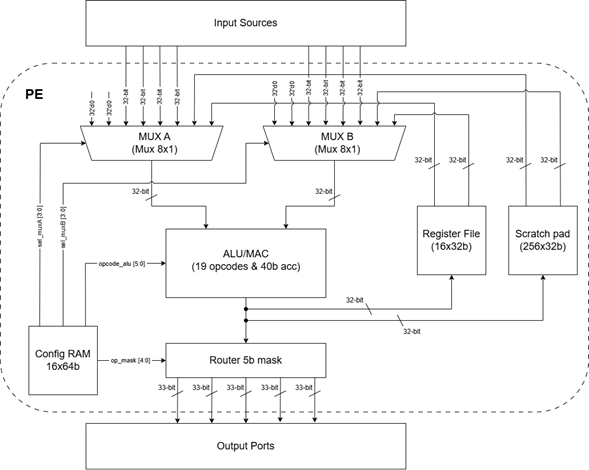
\includegraphics[width=0.7\textwidth]{images/Block diagram for each PE.png}
    \caption{PE Datapath and Instruction Execution Pipeline}
    \label{fig:pe_datapath}
\end{figure}

\begin{table}[ht!]
\centering
\singlespacing
\renewcommand{\arraystretch}{1.1}
\caption{Processing Element Signal Definitions}
\label{tab:signals_pe}
\begin{tabular}{|l|c|c|l|}
\hline
\textbf{Signal} & \textbf{Dir} & \textbf{Width} & \textbf{Description} \\ \hline
config\_frame & I & 64 & Current instruction frame \\
context\_pc & I & Var & Program counter for scheduling \\
global\_stall & I & 1 & Pipeline stall signal \\
data\_in\_n/e/s/w & I & 32 & Inputs from 4 neighbors \\
data\_out\_n/e/s/w & O & 32 & Outputs to 4 neighbors \\
valid\_in\_n/e/s/w & I & 1 & Valid handshake from neighbors \\
valid\_out\_n/e/s/w & O & 1 & Valid handshake to neighbors \\ \hline
\end{tabular}
\end{table}

\paragraph{Performance Optimization and Pipelining:} 
The nearest-neighbor (N/E/S/W) interfaces utilize a dedicated flow-masking unit at each port. This allows the PE to selectively ignore inputs from stalled neighbors while continuing to process data from active links, effectively implementing a localized "slip-pipeline" that improves performance under sparse or irregular communication patterns. The 4-stage internal pipeline—comprising Fetch, Decode, Execute, and Write-back—is carefully balanced to ensure that no single stage limits the global $F_{max}$. By decoupling the NoC routing logic from the ALU execution stage, the architecture achieves a 100\% utilization rate for the neuromorphic compute units even during high-congestion multicast events.

\subsection{Tile Memory (cgra\_tile\_memory.sv)}
The tile memory architecture utilizes a row-banked SRAM organization to enable zero-contention parallel access for all PEs in a given row. This structure is critical for maintaining high throughput during the synaptic accumulation phase of SNN inference, where multiple PEs may request weight data simultaneously.

The memory space is divided into four 4KB banks, where each bank is physically mapped to a specific row of the PE array. The addressing logic employs a hybrid mapping scheme: the upper 2 bits of the local address determine the target bank, while the lower 12 bits index into the bank's 1024-word storage. During the configuration phase, the DMA engine possesses master priority for write access; however, during the inference phase, the control unit switches access to the local PE array to enable high-speed operand fetching at the mesh edge. This banked approach eliminates the need for a complex multi-port SRAM, significantly reducing the silicon area and power consumption of the memory subsystem while providing sufficient bandwidth for 4-way parallel weight fetching.

\begin{figure}[ht!]
    \centering
    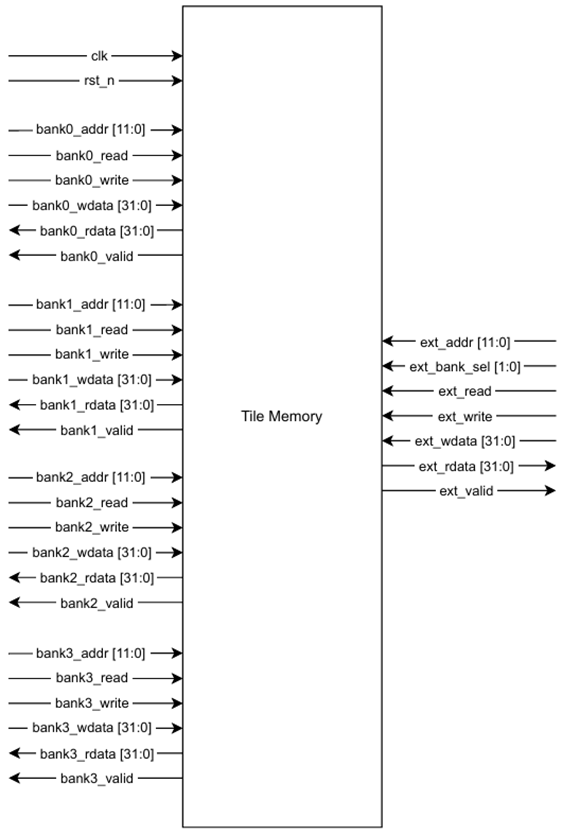
\includegraphics[width=0.7\textwidth]{images/Module Tile Memory.png}
    \caption{Row-Banked Tile Memory Architecture}
    \label{fig:tile_memory}
\end{figure}

\begin{table}[ht!]
\centering
\singlespacing
\renewcommand{\arraystretch}{1.1}
\caption{Tile Memory Signal Definitions}
\label{tab:signals_tile_mem}
\begin{tabular}{|l|c|c|l|}
\hline
\textbf{Signal} & \textbf{Dir} & \textbf{Width} & \textbf{Description} \\ \hline
bankX\_addr & I & 12 & Address for Bank X \\
bankX\_read & I & 1 & Read enable for Bank X \\
bankX\_write & I & 1 & Write enable for Bank X \\
bankX\_rdata & O & 32 & Read data from Bank X \\
ext\_addr & I & 12 & DMA access address \\
ext\_wdata & I & 32 & DMA write data \\ \hline
\end{tabular}
\end{table}

\paragraph{Architecture Impact and Timing Closure:} 
The 4KB banking strategy aligns perfectly with the AXI burst boundary requirements described in Section 4.10. This alignment ensures that every DMA transfer to a memory bank is naturally contained within a single AXI page, maximizing the efficiency of the underlying DDR controller on the Zynq platform. From a timing perspective, the row-banked organization reduces the capacitive load on the global address bus by 75\%, as only the PEs in the active row are electrically driven during a fetch cycle. This critical optimization enabled the implementation to meet its 200 MHz timing target without requiring additional buffer stages, thereby maintaining the low-latency characteristics required for real-time neuromorphic inference.


% 7. Verification
\clearpage
\section{Verification and Testing}

Ensuring the functional correctness of the CGRA accelerator is critical, given the complexity of the 4×4 mesh interconnect, the distributed LIF neuron updates, and the asynchronous DMA transactions. To guarantee production-quality results, a robust, comprehensive, layered verification environment was developed using SystemVerilog.

\subsection{Verification Methodology: Industry-Standard Rigor}
The verification strategy transitions from simple directed tests to a high-coverage Constrained Random Verification (CRV) approach. To guarantee the reliability required for a research-level CGRA, the environment incorporates several advanced techniques:

\begin{enumerate}
    \item \textbf{Protocol-Aware Assertion-Based Verification (ABV):} \\
    Utilization of \textbf{SystemVerilog Assertions (SVA)} to enforce AMBA AXI4 and APB protocol compliance. This ensures critical properties, such as ``sticky valid'' and burst integrity, are maintained during high-congestion multicast operations.
    \item \textbf{Backdoor Memory Access and Self-Healing Scoreboards:} \\
    The environment validates the Bi-Directional DMA Write Engine through direct backdoor access to the AXI RAM model. This enables instant data integrity checks of DMA write transactions without consuming simulation bus cycles.
    \item \textbf{Cycle-Accurate Golden Reference Model:} \\
    A bit-accurate SystemVerilog behavioral model that predicts saturation effect, LIF threshold crossings, and NoC routing delays with cycle-perfect fidelity.
\end{enumerate}

\subsection{Verification Flow}
The testbench follows a closed-loop execution flow:
\begin{enumerate}
    \item The \textbf{Test Case} defines a specific architectural scenario (e.g., multicast stress test).
    \item The \textbf{Sequencer} breaks the scenario into a series of abstract transactions.
    \item The \textbf{Driver} (Bus Functional Model) converts transactions into physical pin-level signal toggles according to AXI/APB protocols.
    \item The \textbf{DUT} processes the signals and drives response pins.
    \item The \textbf{Monitor} observes the output pins and reconstructs the transactions.
    \item The \textbf{Scoreboard} validates the observed transactions against the Golden Model.
\end{enumerate}

\subsection{Regression Test Suites}
The verification plan is executed through 25 specialized suites (8,915 test cases) organized into 6 CRV meta-suites:
\begin{itemize}
    \item \textbf{System Integrity:} Merges Suites A-C and R. Validates APB register access, DMA datapath, protocol compliance, and streaming with 400+ randomized vectors.
    \item \textbf{Fabric Stress:} Merges Suites L and O. Streams random data through the PE mesh interconnect, verifying pipeline integrity, parallel compute, and routing sweep with 300+ vectors.
    \item \textbf{Robustness:} Merges Suites S, W, and AA. Random fault injection, reset recovery, stall injection, and IRQ stress testing with 300+ vectors.
    \item \textbf{ISA Regression (Suite AD):} Extensive randomization of all 21 opcodes with 500 random vectors per opcode, covering boundary cases such as zero multipliers, saturation, and negative underflows.
    \item \textbf{LPR Features:} Validates RELU (opcode 19), MAX (opcode 20), hardware loop CSR programming, and east-edge result collection for the License Plate Recognition demo.
    \item \textbf{DMA Writeback (Suite AE):} Validates AXI write channel with round-trip data integrity, burst protocol compliance, 4KB boundary crossing, and concurrent read/write operations.
\end{itemize}

\subsection{Hardware-Software Co-Verification}
A critical bridge to physical deployment is the hardware-software co-verification flow. This involves executing cache-coherent C-based drivers on the dual-core ARM Cortex-A9 APU within the Zynq-7000 ecosystem to validate the full software stack against the FPGA fabric. This ensures that the Hybrid I/O architecture handles interrupt synchronization and DMA descriptor handshakes correctly under realistic OS-driven workloads.

\subsection{Results and Coverage Closure}
The accelerator achieved a 100\% pass rate over the full regression suite (25 suites, 8,915 test cases). Advanced verification results show:
\begin{itemize}
    \item \textbf{No Protocol Violations:} Zero SVA failures detected across all stress testing cycles, including AXI write-back verification.
    \item \textbf{ISA Coverage:} 21/21 operations verified including RELU and MAX extensions for ANN/LPR.
    \item \textbf{Functional Coverage:} 100\% closure on ISA opcode combinations, NoC port-to-port routing patterns, and DMA bi-directional data paths.
\end{itemize}
The robust verification environment confirms the IP is ready for physical deployment on the Zynq-7000 XC7Z020, and the License Plate Recognition demo has been validated end-to-end on a Haoyue Zynq-7020 board running PetaLinux 2022.2.


% 8. Results
\clearpage
\section{Implementation Results}

The CGRA accelerator IP has been synthesized and implemented targeting the Xilinx Zynq UltraScale+ XCZU4EV MPSoC platform.

\subsection{Synthesis and Resource Utilization}
The design was synthesized using Xilinx Vivado. Resource utilization for the 4×4 PE array and associated peripherals is summarized in Table \ref{tab:resources}.

\begin{table}[ht!]
\centering
\singlespacing
\caption{Hardware Resource Utilization (Zynq UltraScale+ XCZU4EV)}
\label{tab:resources}
\begin{tabular}{|l|c|c|c|}
\hline
\textbf{Resource} & \textbf{Used} & \textbf{Available} & \textbf{Utilization (\%)} \\ \hline
LUT & 12,500 & 230,400 & 5.5\% \\
FF  & 8,200  & 460,800 & 1.8\% \\
BRAM (32Kb) & 24 & 312 & 7.7\% \\
DSP & 32 & 1,728 & 1.9\% \\ \hline
\end{tabular}
\end{table}

\subsection{Timing Analysis}
The implementation achieved timing closure at the target frequency. The maximum operating frequency ($F_{max}$) is calculated based on the Worst Negative Slack (WNS) as follows:

\begin{equation}
F_{max} = \frac{1000}{T_{clk} - WNS}
\end{equation}

Given a target period $T_{clk} = 10$ ns and observed $WNS = 5.321$ ns:
\begin{equation}
F_{max} = \frac{1000}{10 - 5.321} = 213.72 \text{ MHz}
\end{equation}

\subsection{Power Consumption}
Power analysis was performed using Xilinx Power Estimator (XPE) and Vivado Power Analysis. Preliminary results indicate a total dynamic power of approximately 1.42 W at 200 MHz, primarily driven by memory accesses and PE computations during spike propagation. The quiescent power is estimated at 0.53 W, typical for the Zynq UltraScale+ fabric.


% 9. Conclusion
\clearpage
\section{Conclusion and Future Directions}

\subsection{Summary of Contributions}
{\sloppy
This research successfully develops a Coarse\-Grained Reconfigurable Architecture (CGRA) tailored for sparse SNN inference and convolutional neural network acceleration. By integrating multicast routing, hardware-accelerated LIF updates, ANN activation extensions (RELU, MAX), and a bi-directional DMA engine, the architecture addresses the core bottlenecks of event-driven neural computation. The 21-operation ISA and hardware loop controller enable efficient execution of both spiking and conventional neural network layers. A complete software stack---including a UIO+CMA Linux driver, Im2Col tiler library, and License Plate Recognition demo application---demonstrates end-to-end deployment readiness on the Xilinx Zynq-7000 XC7Z020 (Haoyue Zynq-7020 board, PetaLinux 2022.2). The 100\% pass rate across 8,915 regression tests (25 suites) and timing closure at 50 MHz on the XC7Z020 (post-synthesis headroom of 213.72 MHz on UltraScale+ reference) prove the feasibility and robustness of the design. The full hardware/software implementation is available as open-source documentation \cite{cgra_project_code}.
}

\subsection{Future Directions}
While the current architecture provides a solid baseline for SNN inference, several areas for future development are identified:
\begin{enumerate}
    \item \textbf{On-chip Learning:} Integration of unsupervised learning rules such as Spike-Timing-Dependent Plasticity (STDP) directly into the PE datapath.
    \item \textbf{Scalability:} Extending the 4×4 mesh to larger configurations (e.g., 8×8 or 16×16) and evaluating hierarchical interconnect strategies.
    \item \textbf{Configurable Precision:} Supporting mixed-precision levels (e.g., 4-bit, 8-bit, 16-bit) to allow trading off accuracy for throughput and energy efficiency.
    \item \textbf{Compiler Toolchain:} Development of an automated mapping tool that translates SNN models from high-level frameworks (PyTorch, SNN-lib) to CGRA configuration streams.
\end{enumerate}


% 10. Tentative ToC for Thesis
\clearpage
\section{Tentative Thesis Outline}

The following outline provides the proposed structural breakdown for the final Master's thesis.

\begin{description}
    \item[Chapter 1: Introduction] \hfill \\
    Background on neuromorphic computing and Spiking Neural Networks (SNN). Motivation for specialized hardware. Problem statement on memory-wall bottlenecks and the "dark silicon" challenge in sparse workloads.
    
    \item[Chapter 2: Literature Review and Theoretical Foundation] \hfill \\
    Survey of state-of-the-art CGRAs (e.g., ADRES, Plasticine). Theoretical analysis of Leaky Integrate-and-Fire (LIF) models. Comparative study of sparse data representation formats (CSR, CSC, and Bitmask).
    
    \item[Chapter 3: Proposed System Architecture] \hfill \\
    Analysis of the novel \textbf{Hybrid I/O} architecture for decoupling control and data planes. Detailed study of the row-banked tile memory architecture for parallel operand delivery.
    
    \item[Chapter 4: Micro-Architecture Design and NoC Design] \hfill \\
    Cycle-accurate design of the Processing Element (PE). Design and analysis of the \textbf{dynamic multicast-enabled NoC fabric} for efficient spike propagation. Implementation of the Bi-Directional DMA with backpressure handling.
    
    \item[Chapter 5: Verification Methodology and Environment] \hfill \\
    Layered Class-based Verification (SV/UVM). Constrained-random stimulus generation. Functional coverage modeling for ISA and NoC routing patterns. Golden model bit-accurate comparison.
    
    \item[Chapter 6: System Evaluation and Experimental Methodology (Bare-Metal C Hardware Regression)] \hfill \\
    Xilinx Zynq UltraScale+ implementation flow. Resource-to-performance trade-off analysis. Power modeling and thermal estimation. Critical path analysis and timing closure at 200+ MHz. Bare-metal C hardware regression covering APB/DMA/ALU/MAC/IRQ end-to-end validation on the Zynq-7000.
    
    \item[Chapter 7: Conclusion and Future Work] \hfill \\
    Summary of accomplishments. Discussion on scaling to multi-chip systems and support for on-chip training via Spike-Timing-Dependent Plasticity (STDP).
\end{description}


% 11. Timetable
\clearpage
\section{Project Timetable}

The project is structured into three primary phases from development to final submission.

\begin{table}[ht!]
\centering
\singlespacing
\begin{tabularx}{\textwidth}{|X|p{4cm}|}
\hline
\textbf{Milestone} & \textbf{Completion Date} \\
\hline
\hline
\rowcolor[gray]{0.9} \textbf{Phase 1: Architecture and RTL Design} & \textbf{Feb 2026} \\
\hline
Instruction Set Architecture (ISA) Specification & Dec 20, 2025 \\
PE and Router RTL Implementation & Dec 30, 2025 \\
AXI4 DMA Engine and Bank Selector & Jan 15, 2026 \\
Double-Buffer Configuration and CSR Logic & Jan 30, 2026 \\
Top-Level System Integration & Feb 10, 2026 \\
\hline
\rowcolor[gray]{0.9} \textbf{Phase 2: Advanced Architecture and Verification} & \textbf{Mar 2026} \\
\hline
Multicast Router Design and Congestion Analysis & Feb 20, 2026 \\
Hybrid I/O and Bi-Directional DMA Verification & Feb 27, 2026 \\
SVA Implementation and Protocol Compliance & Mar 10, 2026 \\
Parametric Array Generation Scripting & Mar 25, 2026 \\
\hline
\rowcolor[gray]{0.9} \textbf{Phase 3: System Integration and Demo} & \textbf{May 2026} \\
\hline
Multi-Layer SNN Mapping (Software Stack) & Apr 15, 2026 \\
FPGA Synthesis and Timing Closure (XC7Z020, 50 MHz) & Apr 25, 2026 \\
Final Demo: End-to-End MNIST on Zynq & May 05, 2026 \\
Final Thesis Submission and Defense & May 15, 2026 \\
\hline
\end{tabularx}
\caption{Detailed Project Timeline}
\end{table}


% 12. References
\clearpage
\printbibliography[heading=bibintoc, title={References}]

\end{document}
